% Created 2019-07-23 Tue 16:41
% Intended LaTeX compiler: pdflatex
\documentclass[12pt, a4paper]{article}
\usepackage[utf8]{inputenc}
\usepackage[T1]{fontenc}
\usepackage{graphicx}
\usepackage{grffile}
\usepackage{longtable}
\usepackage{wrapfig}
\usepackage{rotating}
\usepackage[normalem]{ulem}
\usepackage{amsmath}
\usepackage{textcomp}
\usepackage{amssymb}
\usepackage{capt-of}
\usepackage{hyperref}
\usepackage[style=authoryear,natbib]{biblatex}
\setlength\bibitemsep{\baselineskip}
\addbibresource{/Users/guilhermesalome/Dropbox/references.bib}
\usepackage[T1]{fontenc}
\usepackage{lmodern}
\usepackage{amsmath}
\usepackage{mathtools}
\usepackage{multirow}
\usepackage{booktabs}
\usepackage{bbm}
\usepackage{dsfont}
\usepackage[]{algorithm2e}
\newcommand\numberthis{\addtocounter{equation}{1}\tag{\theequation}}
\newcommand{\E}[1]{\mathbb{E}{\left[#1\right]}}
\newcommand{\EQ}[1]{\mathbb{E}_t^{\mathbb{Q}}{\left[#1\right]}}
\newcommand{\EP}[1]{\mathbb{E}_t^{\mathbb{P}}{\left[#1\right]}}
\newcommand{\e}[1]{\text{e}^{#1}}
\newcommand{\abs}[1]{\left\vert{#1}\right\vert}
\newcommand{\dis}{\overset{d}{\sim}}
\newcommand{\Var}[1]{\mathrm{Var}\left(#1\right)}
\newcommand{\Corr}[1]{\mathrm{Corr}\left(#1\right)}
\newcommand{\Normal}[1]{\mathcal{N}\left(0, #1\right)}
\newcommand{\stdnormal}{\mathcal{N}\left(0, 1\right)}
\newcommand{\Max}[1]{\text{max}\left\{#1\right\}}
\newcommand{\Set}[1]{\left\{#1\right\}}
\renewcommand{\ln}[1]{\text{ln}\left(#1\right)}
\DeclareMathOperator*{\argmin}{\arg\!\min}
\DeclareMathOperator*{\argmax}{\arg\!\max}
\DeclarePairedDelimiter\ceil{\lceil}{\rceil}
\DeclarePairedDelimiter\floor{\lfloor}{\rfloor}
\newcommand{\Poisson}[1]{\text{Poisson}\left(#1\right)}
\newcommand{\Uniform}[1]{\text{Unif}#1}
\newcommand{\Cov}[1]{\mathrm{Cov}\left(#1\right)}
\newtheorem{problem}{Problem}
\usepackage[hang,small,bf]{caption}
\usepackage[margin=1in]{geometry}
\usepackage{mathtools}
\usepackage{xcolor}
\usepackage{resizegather}
\usepackage{multirow}
\definecolor{darkgreen}{rgb}{0.1, 0.6, 0.1}
\usepackage{float}
\usepackage{setspace}
\usepackage{listings}
\lstdefinestyle{bash}{language=bash,style=Matlab-editor,morekeywords={ssh,cd,pwd,mkdir,ls,man,rmdir,rm,nano,vim,emacs,cat,cp,mv,echo,head,tail,which}}
\definecolor{Code}{rgb}{0,0,0}
\definecolor{Decorators}{rgb}{0.5,0.5,0.5}
\definecolor{Numbers}{rgb}{0.5,0,0}
\definecolor{MatchingBrackets}{rgb}{0.25,0.5,0.5}
\definecolor{Keywords}{rgb}{0,0,1}
\definecolor{self}{rgb}{0,0,0}
\definecolor{Strings}{rgb}{0,0.63,0}
\definecolor{Comments}{rgb}{0,0.63,1}
\definecolor{Backquotes}{rgb}{0,0,0}
\definecolor{Classname}{rgb}{0,0,0}
\definecolor{FunctionName}{rgb}{0,0,0}
\definecolor{Operators}{rgb}{0,0,0}
\definecolor{Background}{rgb}{0.98,0.98,0.98}
\lstdefinelanguage{jupyter-python}{numbers=left, numberstyle=\footnotesize, numbersep=1em, xleftmargin=1em, framextopmargin=2em, framexbottommargin=2em, showspaces=false, showtabs=false, showstringspaces=false, frame=l, tabsize=4, basicstyle=\ttfamily\small\setstretch{1}, backgroundcolor=\color{Background}, commentstyle=\color{Comments}\slshape, stringstyle=\color{Strings}, morecomment=[s][\color{Strings}]{"""}{"""}, morecomment=[s][\color{Strings}]{'''}{'''}, morekeywords={import,from,class,def,for,while,if,is,in,elif,else,not,and,or,print,break,continue,return,True,False,None,access,as,,del,except,exec,finally,global,import,lambda,pass,print,raise,try,assert}, keywordstyle={\color{Keywords}\bfseries}, morekeywords={[2]@invariant,pylab,numpy,np,scipy}, keywordstyle={[2]\color{Decorators}\slshape}, emph={self}, emphstyle={\color{self}\slshape},}
\lstdefinestyle{powershell}{language=bash,style=Matlab-editor,morekeywords={Get-Command}}
\usepackage{fancyhdr}
\pagestyle{fancy}
\fancypagestyle{plain}{}
\fancyhf{}
\rfoot{Page \thepage}
\usepackage{ifthen}
\rhead{\ifthenelse{\value{page}=1}{Guilherme Salom\'{e}}{Summer \the\year}}
\lhead{\ifthenelse{\value{page}=1}{Econ890-04 Python}{Econ890-04 Python}}
\usepackage[numbered,framed]{matlab-prettifier}
\usepackage{listings}
\date{}
\title{Setting Up}
\hypersetup{
 pdfauthor={Guilherme Salomé},
 pdftitle={Setting Up},
 pdfkeywords={},
 pdfsubject={},
 pdfcreator={Emacs 26.1 (Org mode 9.2.1)},
 pdflang={English}}
\begin{document}

\maketitle
To run Python programs all we need is a Python interpreter and a text editor.
In the next section you will learn how to install the reference Python interpreter.
Then we will discuss what IDEs are available for Python.
\section*{Installing Python}
\label{sec:org150c9c9}
The reference Python implementation is CPython.
We will use the 3.6.x version.
The Python 2 version is being discontinued and will soon not be supported anymore, so do not even bother with it.

To install, go to this \href{https://www.python.org/downloads/release/python-368/}{download page for Python 3.6.8}.
On the bottom of the page you will find the links to the installer for different operating systems.
If you are running Windows or MacOS, select the appropriate installer (64-bit) and download it.
Before installing Python read the section bellow for your operating systems.
\subsection*{Windows}
\label{sec:org6d81aa9}
Run the installer, then:
\begin{itemize}
\item In the installation check the boxes: \texttt{Install launcher for all users} and \texttt{Add Python 3.6 to PATH}
\item Then click on \texttt{Install Now}
\item Click on \texttt{Disable path length limit}
\item Finish installing and close the installer
\end{itemize}

Open the Windows \texttt{Power Shell}.
Notice that the power shell is not the same program as the command prompt.
The command prompt is usually a black screen, while the Power Shell will open up a blue screen.

On the \texttt{Power Shell} type:
\lstset{language=bash,label= ,caption= ,captionpos=b,firstnumber=1,numbers=left,style=powershell}
\begin{lstlisting}
# Show where Python was installed
Get-Command py
# Verify that the version of Python is in fact 3.6.x
py --version			# Should print 3.6.x
\end{lstlisting}
The last command should print the correct version of Python that was just installed.
If it does not, then you probably have already installed some other version of Python.
If the version is a recent one, 3.6.x or 3.7.x or higher, then it should be fine.
If it is not, then you will need to either uninstall the previous version and then reinstall Python 3.6.8, or use a virtual environment (discussed in a section below).

You can now launch the Python interpreter by running:
\lstset{language=bash,label= ,caption= ,captionpos=b,firstnumber=1,numbers=left,style=powershell}
\begin{lstlisting}
py
\end{lstlisting}
This will launch Python and you can now type Python commands to have them evaluated just in time.

Notice that Windows refers to Python as \texttt{py}, but all other operating systems use the name \texttt{python} or \texttt{python3}.
For this reason, moving on, we will refer to Python commands that should be run on the Power Shell with \texttt{python} instead of \texttt{py}. But to make the command work in Windows you should write \texttt{py} instead of \texttt{python}.
\subsection*{MacOS}
\label{sec:org9eaabf4}
Run the installer with all defaults.
After installing, open \texttt{Terminal} and verify the installation:
\lstset{language=bash,label= ,caption= ,captionpos=b,firstnumber=1,numbers=left,style=bash}
\begin{lstlisting}
# Show where Python was installed
which python
# Verify that the version of Python is in fact 3.6.x
python --version
\end{lstlisting}
MacOS usually comes with a Python 2.x preinstalled, so the command above might return something like \texttt{Python 2.7.10}.
However, you can still access the Python you just installed with the command \texttt{python3} or even \texttt{python3.6}.
To verify this is the case, run the following on \texttt{Terminal}:
\lstset{language=bash,label= ,caption= ,captionpos=b,firstnumber=1,numbers=left,style=bash}
\begin{lstlisting}
python3 --version
\end{lstlisting}
And you should get back \texttt{Python 3.6.8}.

You can now launch the Python interpreter by running:
\lstset{language=bash,label= ,caption= ,captionpos=b,firstnumber=1,numbers=left,style=bash}
\begin{lstlisting}
python3
\end{lstlisting}
This will launch Python and you can now type Python commands to have them evaluated just in time.

Moving on, whenever you see a command for \texttt{Terminal} starting with \texttt{python}, please make the substitution to \texttt{python3}.
\subsection*{GNU/Linux}
\label{sec:org55077fd}
To install Python on GNU/Linux, open \texttt{Terminal} and run:
\lstset{language=bash,label= ,caption= ,captionpos=b,firstnumber=1,numbers=left,style=bash}
\begin{lstlisting}
# Update source list
sudo apt-get update
# Install Python 3.6
sudo apt-get install python3.6
sudo apt-get install python3-pip
\end{lstlisting}
Now, check if we got the correct version installed by typing the following:
\lstset{language=bash,label= ,caption= ,captionpos=b,firstnumber=1,numbers=left,style=bash}
\begin{lstlisting}
python --version
\end{lstlisting}
On GNU/Linus you may already have a Python 2 installed, so Python 3.6 would be available as \texttt{python3} or even \texttt{python3.6} instead.
If the command above does not return \texttt{Python 3.6.x}, then try the following:
\lstset{language=bash,label= ,caption= ,captionpos=b,firstnumber=1,numbers=left,style=bash}
\begin{lstlisting}
python3 --version
# or
python3.6 --version
\end{lstlisting}
And you should see \texttt{Python 3.6}.

You can now launch the Python interpreter by running:
\lstset{language=bash,label= ,caption= ,captionpos=b,firstnumber=1,numbers=left,style=bash}
\begin{lstlisting}
python3
\end{lstlisting}
This will launch Python and you can now type Python commands to have them evaluated just in time.

Moving on, whenever you see a command for \texttt{Terminal} starting with \texttt{python}, please make the appropriate substitution to \texttt{python3} or \texttt{python3.6}.
\section*{Python Package Installer}
\label{sec:orga74b61e}
Now, we need to install the Python Package Installer, also known as \texttt{pip}, which is responsible for downloading and installing additional packages that we might require.
To do so, run the following in the \texttt{Terminal} (or \texttt{Power Shell}):
\lstset{language=bash,label= ,caption= ,captionpos=b,firstnumber=1,numbers=left,style=bash}
\begin{lstlisting}
python -m pip install -U pip
\end{lstlisting}
Remember to make the appropriate substitution of \texttt{python} so that you are using Python 3 and not Python 2.

The command above will install and upgrade \texttt{pip} to the latest version.
You can now use \texttt{pip} to install packages.

The packages installed using \texttt{pip} are fetched from a central repository called the Python Package Index (PyPI, \url{https://pypi.org}).
These packages are installed in a folder named \texttt{site-packages}, and the packages are local to each version of Python (more about this on the section about virtual environments).

Packages can be installed with the command \texttt{pip install <package\_name>}, and uninstalled with \texttt{pip uninstall <package\_name>}.
In some systems, it is not possible to call \texttt{pip} directly, so you should run instead:
\lstset{language=bash,label= ,caption= ,captionpos=b,firstnumber=1,numbers=left,style=bash}
\begin{lstlisting}
python -m pip install <package_name>
\end{lstlisting}
The command \texttt{pip list} lists all installed packages and their version numbers.
The command \texttt{pip list -{}-outdated} shows installed packages that are outdated.
Outdated packages can be updated with \texttt{pip install -{}-upgrade <outdate\_package\_name>}.
The command \texttt{pip show <package\_name>} gives a detailed description of the installed package, including where it is installed, the version number and dependencies.

An important feature of \texttt{pip} is that it can install packages listed in a file automatically. Why is this useful? Let's say you are working on a research project, and end up installing 20 different packages. Then, you need to share your code with a co-author or you need to run your code on a faster computer. Then you need to find out what were all of the 20 packages you installed and what were their versions, since using very different versions of packages could break your code.
Fortunately, \texttt{pip} makes this task easy:
\lstset{language=bash,label= ,caption= ,captionpos=b,firstnumber=1,numbers=left,style=bash}
\begin{lstlisting}
pip freeze > requirements.txt
\end{lstlisting}
The command above will create a text file containing a list of all the packages you have installed and their versions. Each line will contain a single package and the version number.
You can send this file to your co-author or new computer and run:
\lstset{language=bash,label= ,caption= ,captionpos=b,firstnumber=1,numbers=left,style=bash}
\begin{lstlisting}
pip install -r requirements.txt
\end{lstlisting}
The command will install all of the packages in the same versions you were originally using.
\section*{Text Editors and Integrated Development Environments (IDEs)}
\label{sec:org51856e2}
To write Python programs we need to write commands in a text file ending in \texttt{.py}.
Then we tell Python to execute the commands in that file.
In order to help us write those files, it is useful to have a text editor that has syntax highlighting and auto completion of certain terms.

Below is a short list of possible text editors that you can use:
\begin{itemize}
\item Editors/IDEs that are \uline{easy} to setup and use:
\begin{itemize}
\item Any text editor, like TextEdit or Notepad. The caveat with these editors is that there is no syntax highlighting or other utilities.
\item \href{https://docs.python.org/3/library/idle.html}{IDLE}: comes installed with Python. Provides a simple editor and Python shell.
\item \href{https://www.anaconda.com/distribution/}{Anaconda} is a full IDE that comes with many packages preinstalled (it also comes with Jupyter, mentioned in the list below). It is open source and free to use. Most beginners to Python use this distribution. It provides an environment similar to Matlab or R, with a text editor and a REPL. Installing Anaconda will install Python in a virtual environment so that it is separate from the Python in your system. More about virtual environments in the sections below.
\end{itemize}
\item Editors/IDEs that are \uline{medium difficulty} to setup and use:
\begin{itemize}
\item \href{https://jupyter.org}{Jupyter Notebook}: it is a web application for creating documents that mix text, images and code. It is open source and free to use. We will use this IDE to code during most of the lectures.
\item \href{https://code.visualstudio.com}{Visual Studio Code}: an IDE by Microsoft. You can add support for Python within the program. It is free to use and can be customized.
\item \href{https://atom.io}{Atom}: an IDE created by people at Github. You can add support for Python installing packages such as \href{https://atom.io/packages/ide-python}{this}. It can be customized with JavaScript.
\item \href{https://www.sublimetext.com}{Sublime}: paid text editor. Can be used for Python with plugin.
\end{itemize}
\item Editors/IDEs that are \uline{hard} to setup and use:
\begin{itemize}
\item \href{https://www.gnu.org/software/emacs/}{GNU Emacs}: a customizable text editor. Can be made into an IDE for Python with packages such as \href{https://github.com/jorgenschaefer/elpy\#elpy-the-emacs-lisp-python-environment}{Elpy}.
\item \href{https://www.vim.org}{Vim}: a customizable text editor. Can be made into an IDE for Python by following \href{https://realpython.com/vim-and-python-a-match-made-in-heaven/}{this tutorial}.
\end{itemize}
\end{itemize}

If you write a lot of Python code, you should think about learning how to use Emacs or Vim, since they are incredible text editors (but with a steep learning curve). Anaconda is a very good IDE for beginners and comes with most of the packages we will use preinstalled, including Jupyter.
Jupyter Notebook is great for sharing code with others during presentations (or discussions with faculty).
During the lectures we will use Jupyter Notebook as our Python IDE, but when you are coding by yourself you may want to use something else.
Feel free to use whatever editor you are most comfortable with.
\section*{Virtual Environments}
\label{sec:orgfc1cc95}
So far we have installed Python 3.6.8 in our computer and also the package Jupyter Notebook.
You probably have run into the issue that another version of Python was already installed on your system, most likely Python 2.
And that to access the correct version of Python we had to be careful and use \texttt{python3} or \texttt{python3.6}.
To avoid having to deal with these issues we will create something called a virtual environment.

To understand what a virtual environment is, we need to understand how your computer finds a program when you type \texttt{python} in the \texttt{Terminal}.
When we tell the terminal to run a program, it tries to find the program in a list of folders.
This list of folders is stored in a variable named \texttt{PATH}.
You can see this list by typing the following in the \texttt{Terminal}:
\lstset{language=bash,label= ,caption= ,captionpos=b,firstnumber=1,numbers=left,style=bash}
\begin{lstlisting}
echo $PATH
\end{lstlisting}
In \texttt{Power Shell}:
\lstset{language=bash,label= ,caption= ,captionpos=b,firstnumber=1,numbers=left,style=powershell}
\begin{lstlisting}
$Env: Path
\end{lstlisting}
You will get a list like this:
\lstset{language=bash,label= ,caption= ,captionpos=b,firstnumber=1,numbers=left,style=bash}
\begin{lstlisting}
/usr/local/bin:/usr/bin:/bin:/usr/sbin:/sbin
\end{lstlisting}
The folders are separated by colons, and the search for the program follows the order of the folders in the list.
In this case, if we type \texttt{python}, we will search for the program \texttt{python} in the folder \texttt{/usr/local/bin}, since my Python 3.6.x is installed in that folder it will be found and executed.
This is why, in my computer when I type \texttt{which python}, I get back \texttt{Python 3.6}.
Now, if I did not have Python 3.6 installed, then there would be no \texttt{python} in the folder \texttt{/usr/local/bin} and the search would fail.
We would then search for \texttt{python} in \texttt{/usr/bin} where we would find it.
In my computer, the \texttt{python} inside \texttt{/usr/bin} is the Python installed with the operating system (Python 2.7.10).

What would happen if we switched the order of folders in \texttt{PATH} to the following:
\lstset{language=bash,label= ,caption= ,captionpos=b,firstnumber=1,numbers=left,style=bash}
\begin{lstlisting}
/usr/bin:/usr/local/bin:/bin:/usr/sbin:/sbin
\end{lstlisting}
And then typed:
\lstset{language=bash,label= ,caption= ,captionpos=b,firstnumber=1,numbers=left,style=bash}
\begin{lstlisting}
which python			# Get-Command py in Windows
\end{lstlisting}
What should be the result of the command above?
It would print out \texttt{Python 2.7.10}, since it would search for \texttt{python} now starting in the \texttt{/usr/bin} folder instead of \texttt{/usr/local/bin}.
Therefore, changing the order of folders in \texttt{PATH} changes where the system will search for programs to run.

What a virtual environment does is temporarily modify the list of folders in \texttt{PATH}, so that if we type \texttt{python} we get the Python version we expect to get, no matter where it is.
\section*{Creating a Virtual Environment for Python}
\label{sec:org301cbeb}
There are many ways to create a virtual environment, here we will use the package \texttt{virtualenv}.
This package creates an isolated Python environment in a folder.
We can activate this environment so that \texttt{python} points to the Python installed in that folder.
This also means that packages installed with \texttt{pip} will be installed for the Python in that folder.
This isolates Python in a way that is easy to replicate and control.

Install \texttt{virtualenv} with \texttt{pip}:
\lstset{language=bash,label= ,caption= ,captionpos=b,firstnumber=1,numbers=left,style=bash}
\begin{lstlisting}
python3 -m pip install virtualenv
\end{lstlisting}
Next, we will call \texttt{virtualenv} with two arguments.
The first argument is the path to the folder where we want to create the virtual environment.
The second argument is the python version we want to install in that environment.
Run the following:
\lstset{language=bash,label= ,caption= ,captionpos=b,firstnumber=1,numbers=left,style=bash}
\begin{lstlisting}
virtualenv ~/Desktop/py36 --python=python3.6
\end{lstlisting}
If you are a Windows user and you get an error message about "Execution Policy", then you should read the blue \texttt{Note} box in \href{https://virtualenv.pypa.io/en/latest/userguide/}{this page}.

At this point \texttt{virtualenv} has created a folder \texttt{py36}. Its contents are:
\lstset{language=bash,label= ,caption= ,captionpos=b,firstnumber=1,numbers=left,style=bash}
\begin{lstlisting}
py36/
|-- bin/      # contains python and pip binaries, and activate script
|-- include/  # C code used by Python
|-- lib/      # python packages: standard library and downloads
    |-- python3.6/
        |-- site-packages/ # packages installed with pip go here
\end{lstlisting}
If you are a Windows user, then you should see similar folders and a folder named \texttt{Scripts}.

To actually make the virtual environment active, execute the following:
\lstset{language=bash,label= ,caption= ,captionpos=b,firstnumber=1,numbers=left,style=bash}
\begin{lstlisting}
source ~/Desktop/py36/bin/activate
\end{lstlisting}
In \texttt{Power Shell}:
\lstset{language=bash,label= ,caption= ,captionpos=b,firstnumber=1,numbers=left,style=powershell}
\begin{lstlisting}
. ~\Desktop\py36\Scripts\activate.ps1
\end{lstlisting}
This script will activate the virtual environment, making the necessary changes to the \texttt{PATH} variable, so that typing \texttt{python} just works.

We can check that we are calling the right Python by running:
\lstset{language=bash,label= ,caption= ,captionpos=b,firstnumber=1,numbers=left,style=bash}
\begin{lstlisting}
which python                    # returns ~/Desktop/py36/bin/python
python --version                # returns Python 3.6.8
echo $PATH			# notice what is the first folder in the list!
\end{lstlisting}
Now we can run our Python code, install packages and everything related to Python will be contained in the \texttt{py36} folder.
We localized Python 3.6 and any packages we install to the \texttt{py36} folder.
Because we are using the virtual environment, we do not need to remember to make the appropriate substitution of \texttt{python} for \texttt{python3} or \texttt{python3.6} anymore.

After you are done working with Python 3.6 you can simply run \texttt{deactivate} to exit the virtual environment (or just close the terminal).

Notice that your programs do not need to necessarily be on the \texttt{py36} folder.
That folder simply contains Python and packages that we will use when the environment is active.
The IDE Anaconda creates a virtual environment with Python and other packages under the hood, basically replicating the process we above.
\section*{Installing Jupyter Notebook}
\label{sec:org47b97b1}
We will now install Jupyter Notebook, which is the web browser based IDE we are going to use during the lectures.
To do so, first activate the virtual environment so that we install Jupyter for the right version of Python.
\lstset{language=bash,label= ,caption= ,captionpos=b,firstnumber=1,numbers=left,style=bash}
\begin{lstlisting}
source ~/Desktop/py36/bin/activate
\end{lstlisting}
To install Jupyter Notebook we can use \texttt{pip}. Run the following in a \texttt{Terminal} (or \texttt{Power Shell} for Windows users):
\lstset{language=bash,label= ,caption= ,captionpos=b,firstnumber=1,numbers=left,style=bash}
\begin{lstlisting}
pip install jupyter
\end{lstlisting}
Now you have installed Jupyter Notebook.
To run the notebook, simply type:
\lstset{language=bash,label= ,caption= ,captionpos=b,firstnumber=1,numbers=left,style=bash}
\begin{lstlisting}
jupyter notebook
\end{lstlisting}
This will start the jupyter notebook server on your terminal and then launch a browser with the Jupyter Notebook application.
There you can create a new file and start coding.
To shutdown the notebook just go back to the Terminal and hit Ctrl-C twice.
\section*{Preparing For the Next Lectures}
\label{sec:orgfff56d0}
At the beginning of each lecture, the first thing you should do is activate the virtual environment:
\lstset{language=bash,label= ,caption= ,captionpos=b,firstnumber=1,numbers=left,style=bash}
\begin{lstlisting}
source ~/Desktop/py36/bin/activate
\end{lstlisting}
We will also create a folder to hold all of our lecture notes:
\lstset{language=bash,label= ,caption= ,captionpos=b,firstnumber=1,numbers=left,style=bash}
\begin{lstlisting}
# Create a directory to hold lectures
mkdir ~/Desktop/python_course
cd  ~/Desktop/python_course
# in Bash this can be done in one line
mkdir ~/Desktop/python_course && cd "$_"
# $_ is a special symbol that captures the arguments of the last command
# we add quotes around it to deal with possible spaces in the name
\end{lstlisting}
Finally, you should launch Jupyter Notebook:
\lstset{language=bash,label= ,caption= ,captionpos=b,firstnumber=1,numbers=left,style=bash}
\begin{lstlisting}
# Launch jupyter notebook
jupyter notebook
\end{lstlisting}
At each lecture we will code in Python using Jupyter notebooks, one for each topic.
When you download Jupyter notebooks from the course website, you will get files ending in \texttt{.ipynb}.
Put these files in the folder \texttt{python\_course} you just created, and when you launch \texttt{jupyter notebook} from that folder, you should see those files in your browser.
If you click on a file, a new tab will open and you can start coding.
\section*{Jupyter Notebook Basics}
\label{sec:org0c3e5c9}
Jupyter notebook is a software (web application) that facilitates sharing interactive documents, referred to as jupyter notebooks.
We will use these notebooks to learn Python.
We can use jupyter notebooks to write code, execute it and interact with its outputs.
Next, we discuss the basics of Jupyter Notebook.

Launch Jupyter Notebook in the \texttt{python\_course} folder:
\lstset{language=bash,label= ,caption= ,captionpos=b,firstnumber=1,numbers=left,style=bash}
\begin{lstlisting}
source ~/Desktop/py36/bin/activate
cd ~/Desktop/python_course
jupyter notebook
\end{lstlisting}
Your browser should open a new tab with Jupyter Notebook (see Figure \ref{fig:org3cb8600}).

\begin{figure}[htbp]
\centering
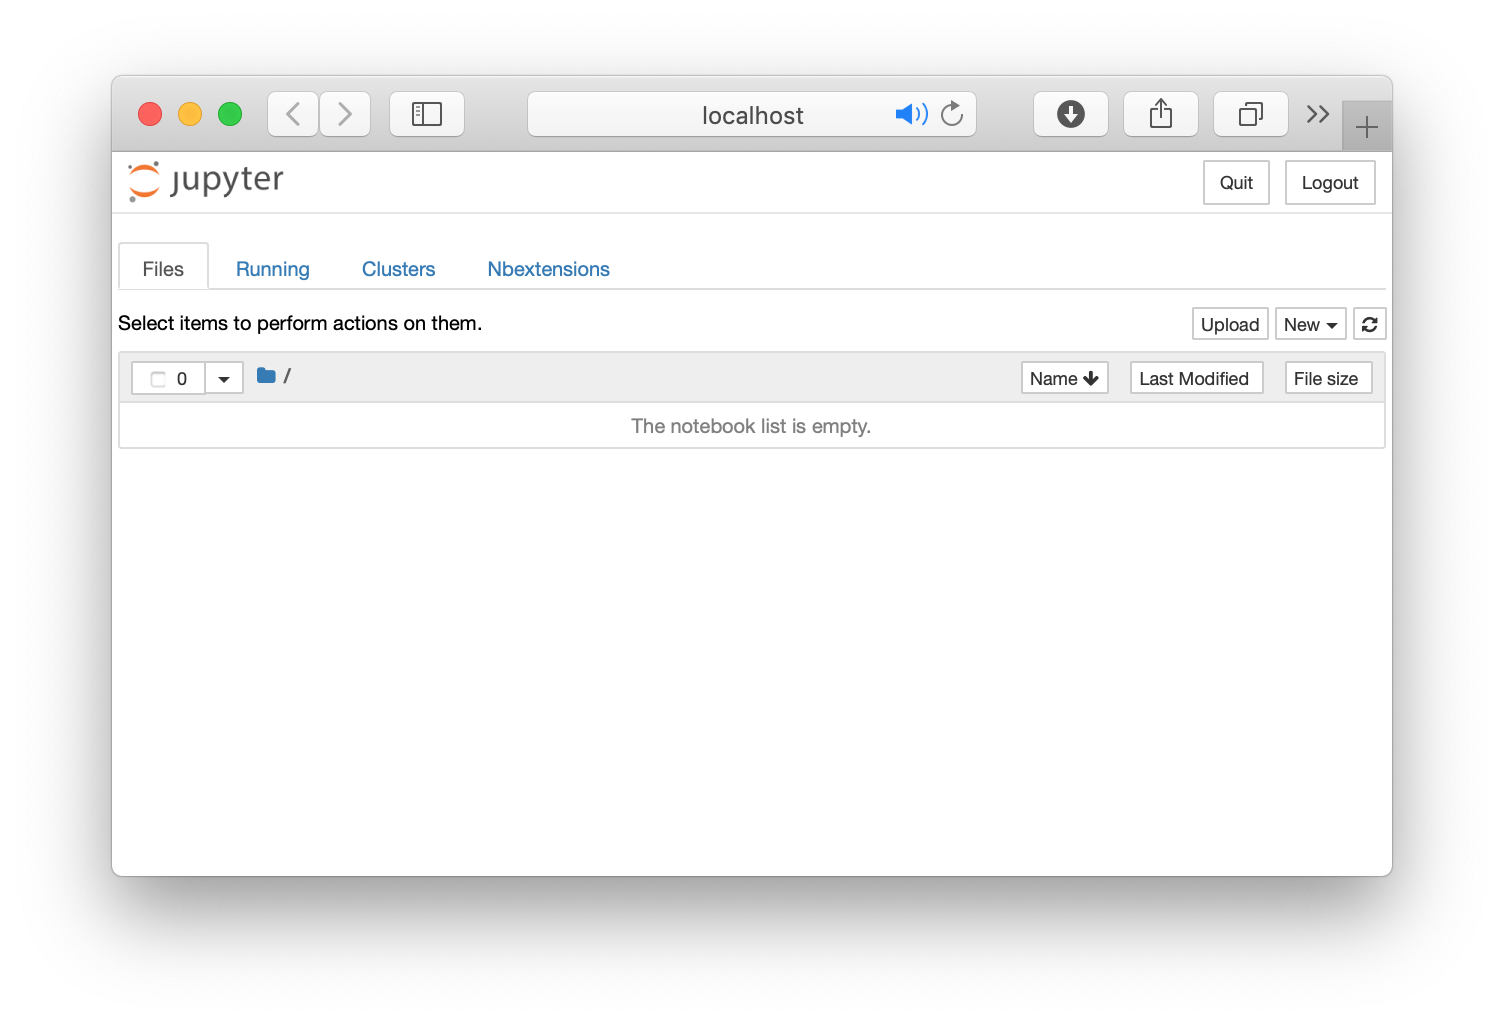
\includegraphics[width=.9\linewidth]{/Users/guilhermesalome/Teaching/Duke/Econ890 Python - 2019/supporting/python_jupyter_notebook.png}
\caption{\label{fig:org3cb8600}
Launching Jupyter Notebook for the First Time on an Empty Folder.}
\end{figure}

Create a new notebook by clicking on the \texttt{New} button and then selecting \texttt{Python 3} (see Figure \ref{fig:org787f0a9}).
\begin{figure}[htbp]
\centering
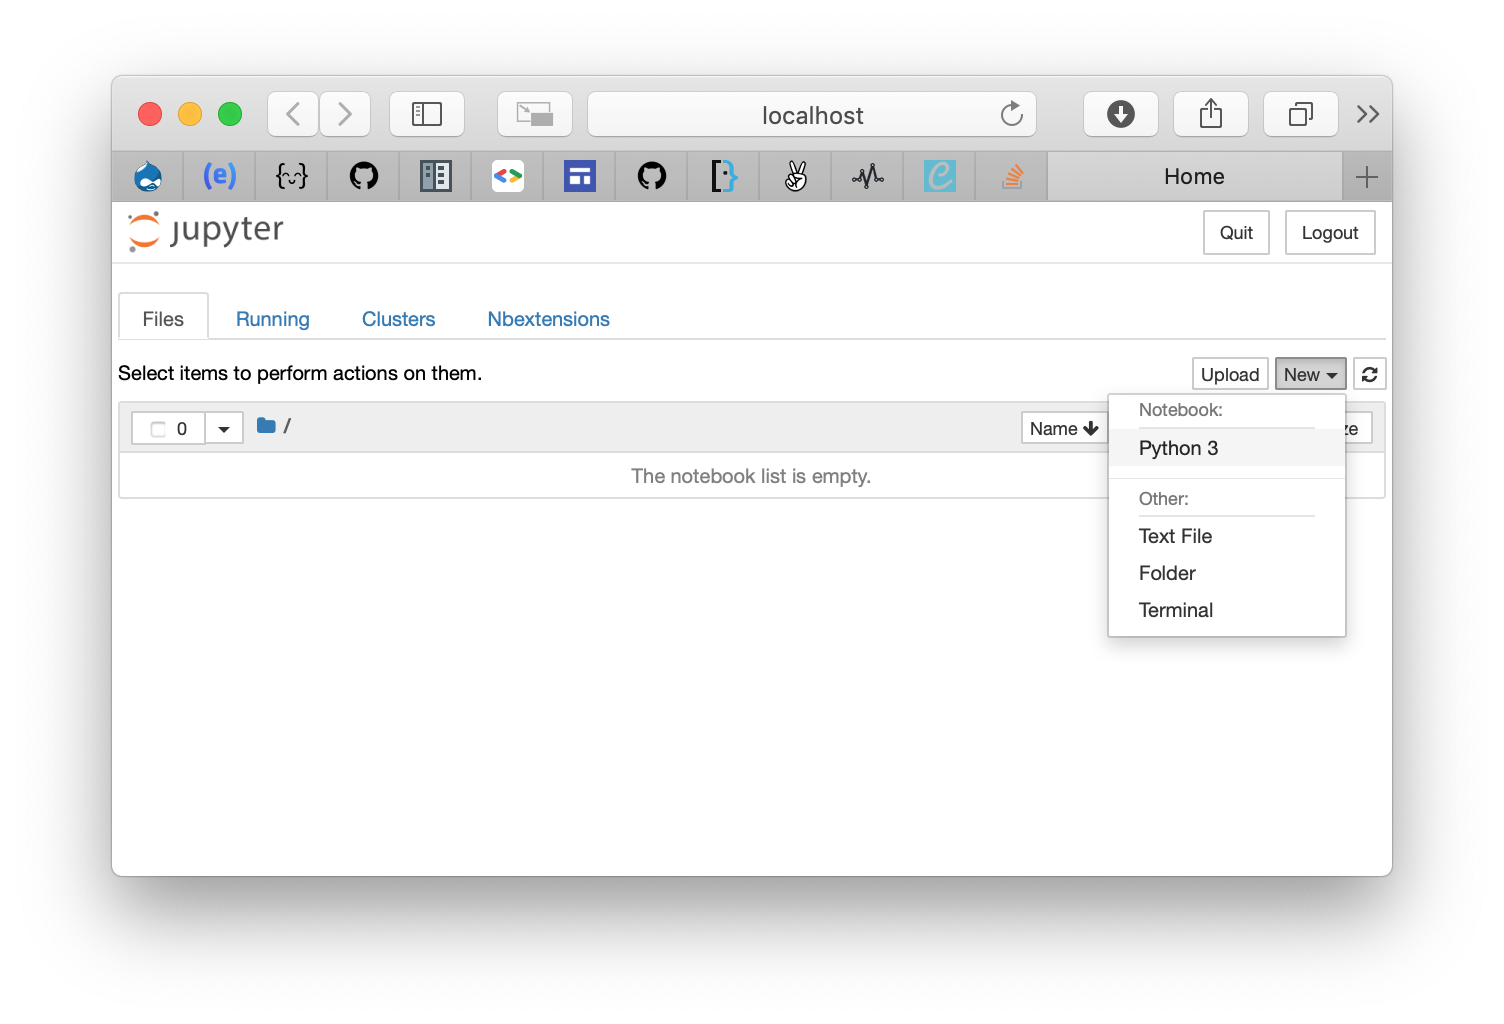
\includegraphics[width=.9\linewidth]{/Users/guilhermesalome/Teaching/Duke/Econ890 Python - 2019/supporting/python_jupyter_create_new_notebook.png}
\caption{\label{fig:orge8584c8}
Creating a new notebook.}
\end{figure}

The notebook will open in a new tab (see Figure \ref{fig:org787f0a9}).

\begin{figure}[htbp]
\centering
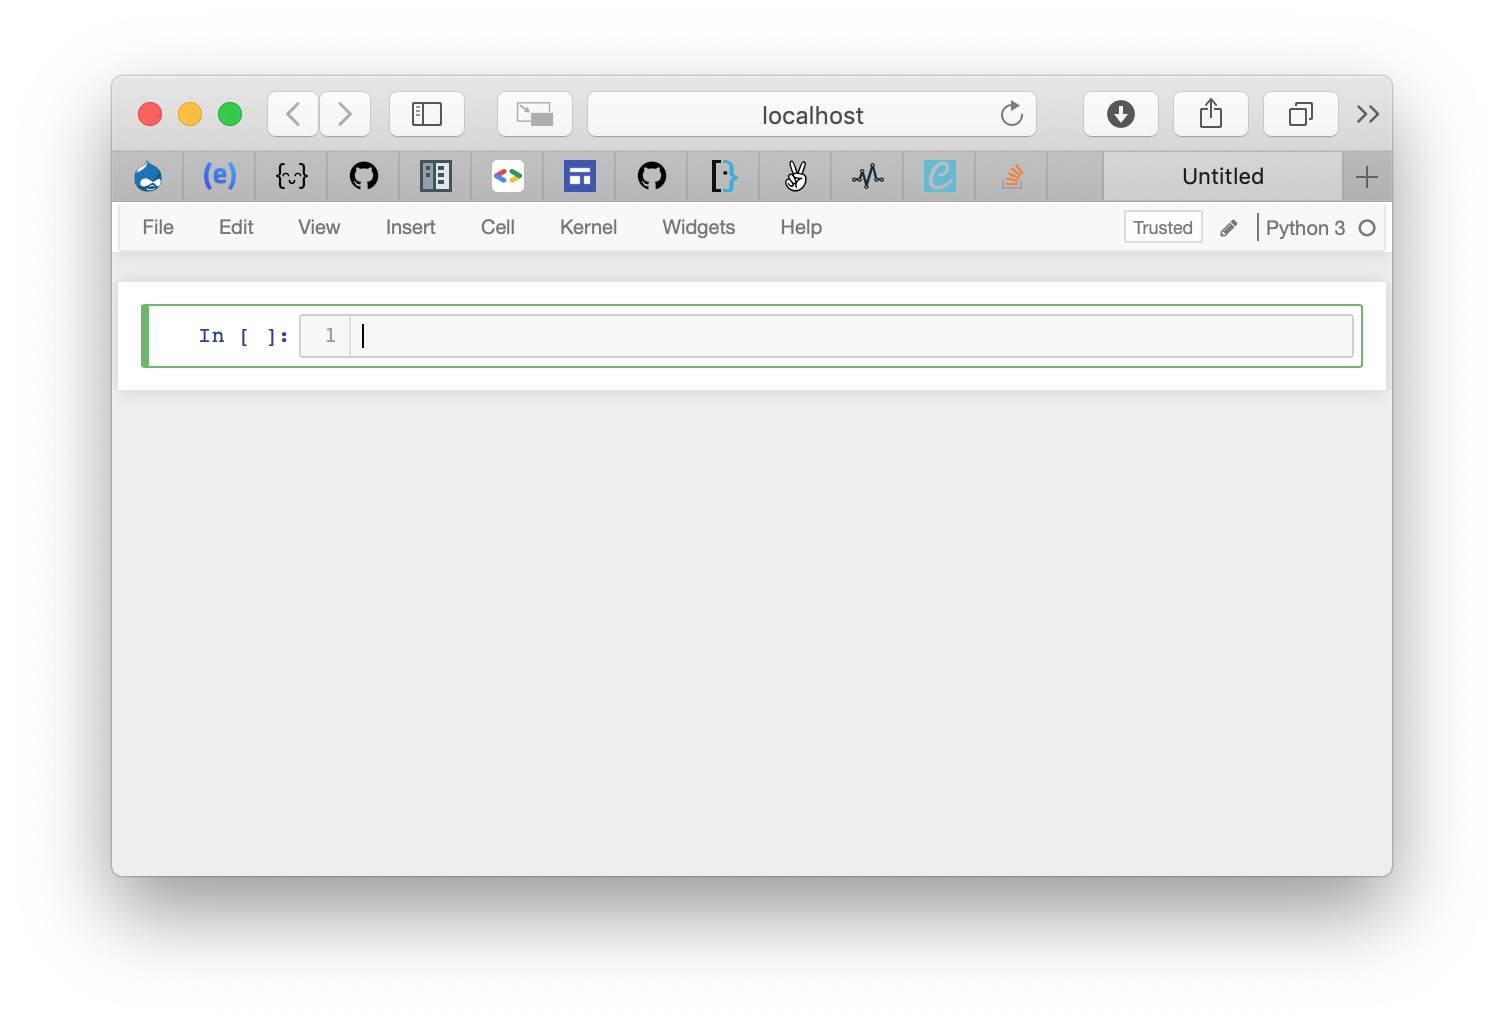
\includegraphics[width=.9\linewidth]{/Users/guilhermesalome/Teaching/Duke/Econ890 Python - 2019/supporting/python_jupyter_new_notebook.png}
\caption{\label{fig:org787f0a9}
A new jupyter notebook.}
\end{figure}

The box you see on the screen is called a \texttt{cell}.
There are two types of cells: code cells and markdown cells.

On code cells you can type Python code.
Go ahead and type \texttt{print("Hello World!")}.
We can execute the code by going on the menu \texttt{Cell} and clicking on the button \texttt{Run Cells}.
This will run the Python code you just typed, and the output of this code, if any, will be displayed right below the code (see Figure \ref{fig:org9a6797a}).
Alternatively, you can run the code with the shortcut \texttt{Ctrl-Enter}.
You can also run the code in the cell with the shortcut \texttt{Shift-Enter}.
Pressing \texttt{Shift-Enter} will run the code, output its results, and create a new code cell below the one you just executed.

\begin{figure}[htbp]
\centering
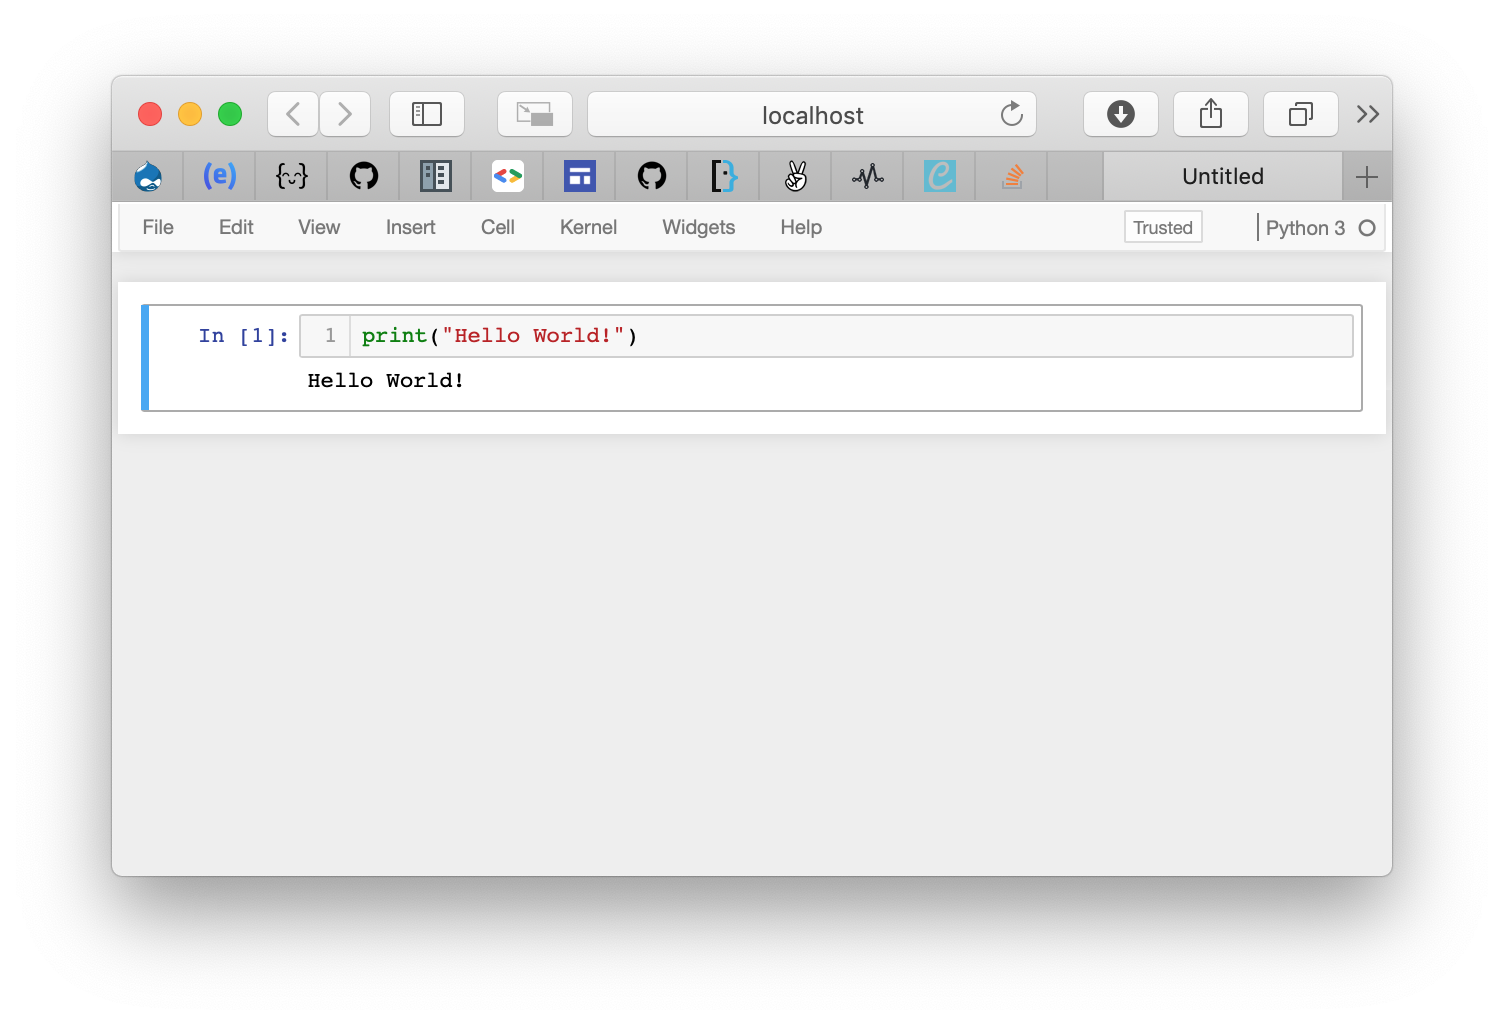
\includegraphics[width=.9\linewidth]{/Users/guilhermesalome/Teaching/Duke/Econ890 Python - 2019/supporting/python_hello_world.png}
\caption{\label{fig:org9a6797a}
Running Python code in a Code Cell.}
\end{figure}

Notice that after hitting \texttt{Shift-Enter}, you get a new code cell, and its left side has a blue vertical bar (see Figure \ref{fig:org0fe2f02}).

\begin{figure}[htbp]
\centering
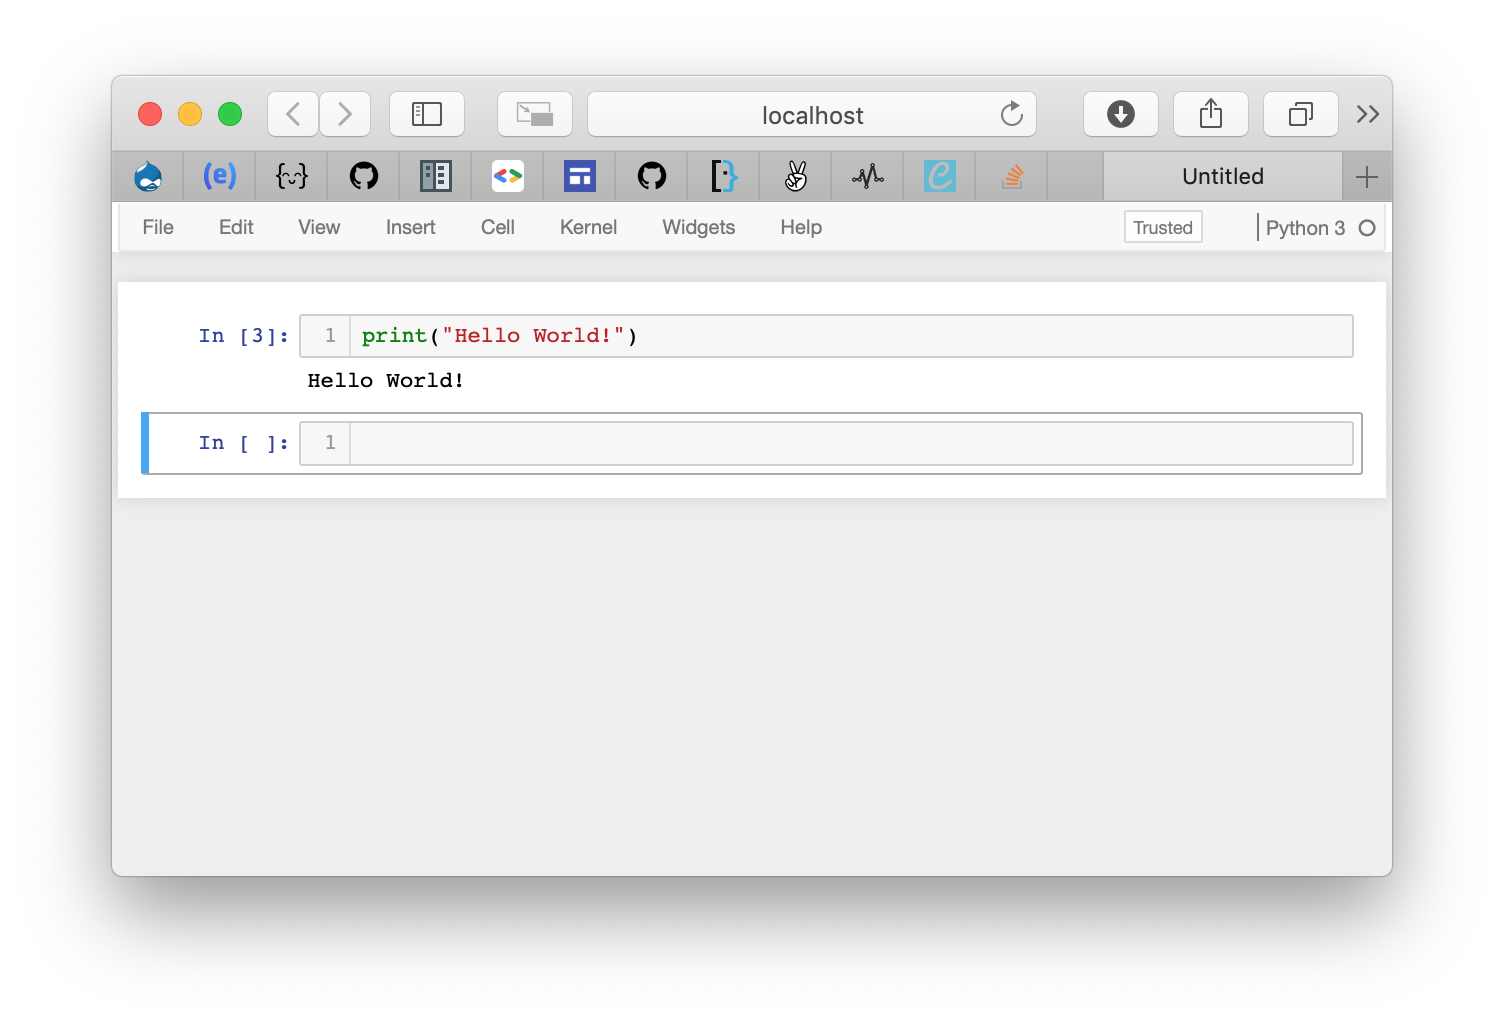
\includegraphics[width=.9\linewidth]{/Users/guilhermesalome/Teaching/Duke/Econ890 Python - 2019/supporting/python_blue_code_cell.png}
\caption{\label{fig:org0fe2f02}
Code Cell in Command Mode.}
\end{figure}

When the cell is in blue, we are in \texttt{Command Mode}.
This means we can use some shortcuts to move between cells and other functionality.
If you hit \texttt{Enter}, then you will go inside the cell and you are now in \texttt{Edit Mode}.
Notice that the left side of the cell is now green.
In this mode, you can type text inside the cell, and other shortcuts are available.
You can exit \texttt{Edit Mode} to \texttt{Command Mode} by hitting \texttt{ESC}.

\begin{figure}[htbp]
\centering
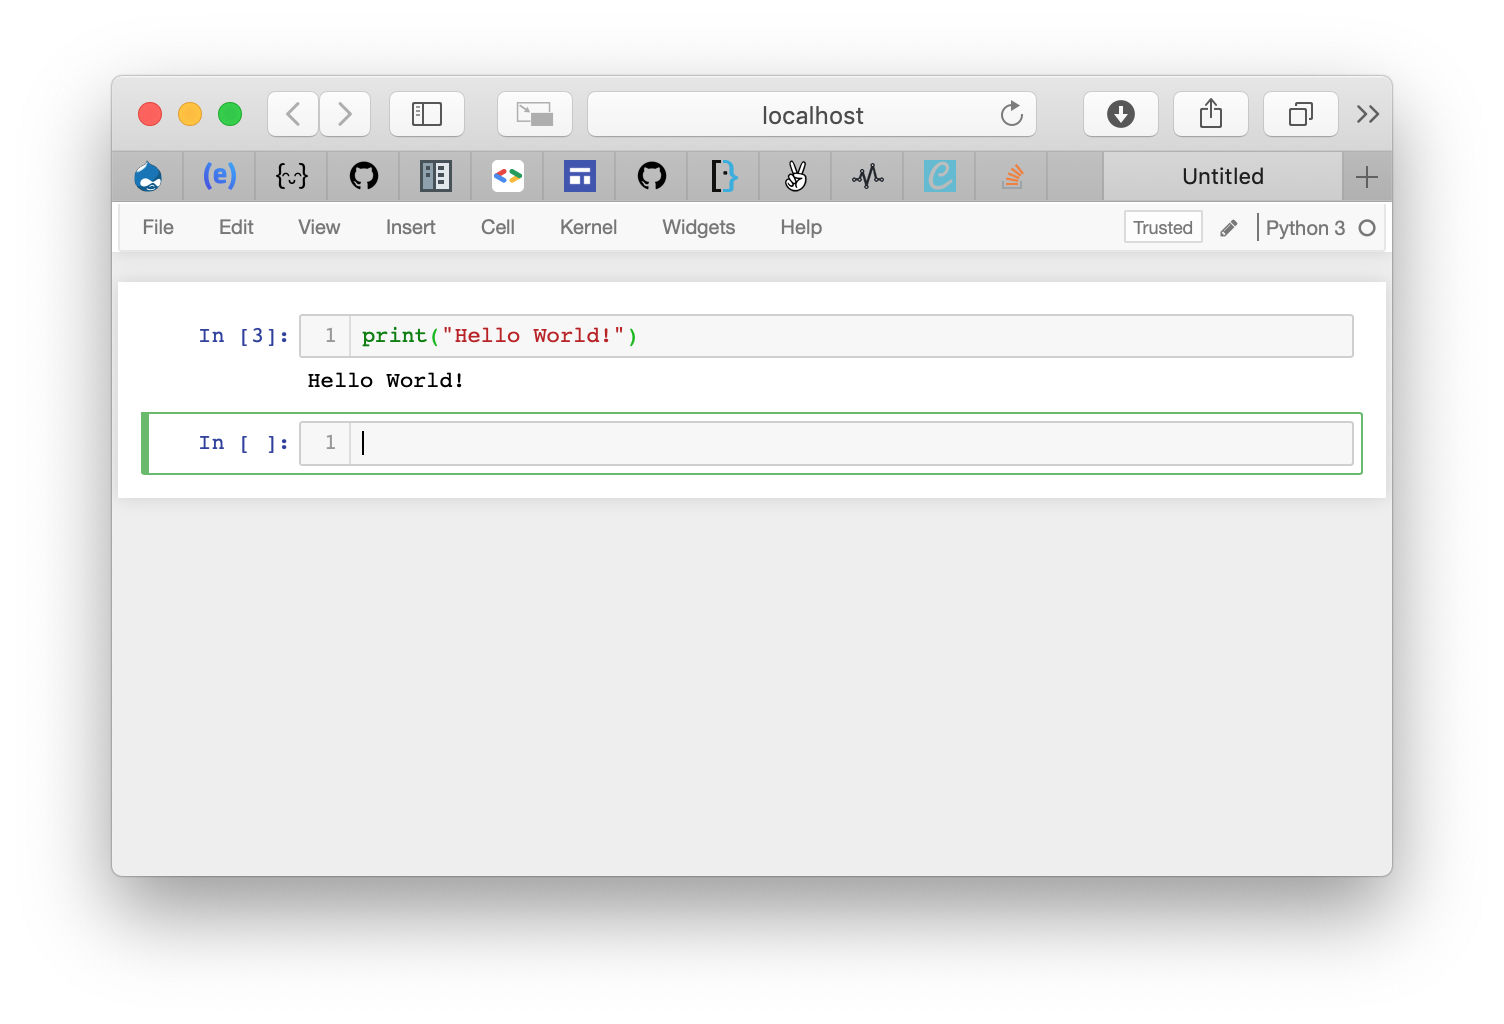
\includegraphics[width=.9\linewidth]{/Users/guilhermesalome/Teaching/Duke/Econ890 Python - 2019/supporting/python_green_code_cell.png}
\caption{\label{fig:org939f7c7}
Code Cell in Edit Mode.}
\end{figure}

We can change a code cell into a markdown cell by hitting \texttt{m} (for markdown) while on \texttt{Command Mode}.
Notice that now the word \texttt{In [ ]:} disappears from the cell.
The markdown cell is a cell that holds rich text, supports the \href{https://www.markdownguide.org/basic-syntax}{Markdown markup language}, and also Latex.
We can use these cells to write information relevant to understand the code in code cells.
Go into \texttt{Edit Mode} and type the following in the markdown cell:

\begin{verbatim}
A markdown cell holds text.
We can use the Markdown markup language to format the text.
For example:
- **bold text** is created by surrounding text with double asterisks: **.
Markdown cells also support Latex:
- In-line equations: $f(x)=x^2$
- We can also use some environments, like align:
\begin{align}
f(x) &= x^2\\\\
g(x) &= x^3
\end{align}
\end{verbatim}

Now, hit \texttt{Control-Enter} to execute the markdown cell.
This will format the text, taking care of the Markdown formatting and the Latex, and the output will be displayed in the cell (see Figure \ref{fig:orgdf01b9d}).

\begin{figure}[htbp]
\centering
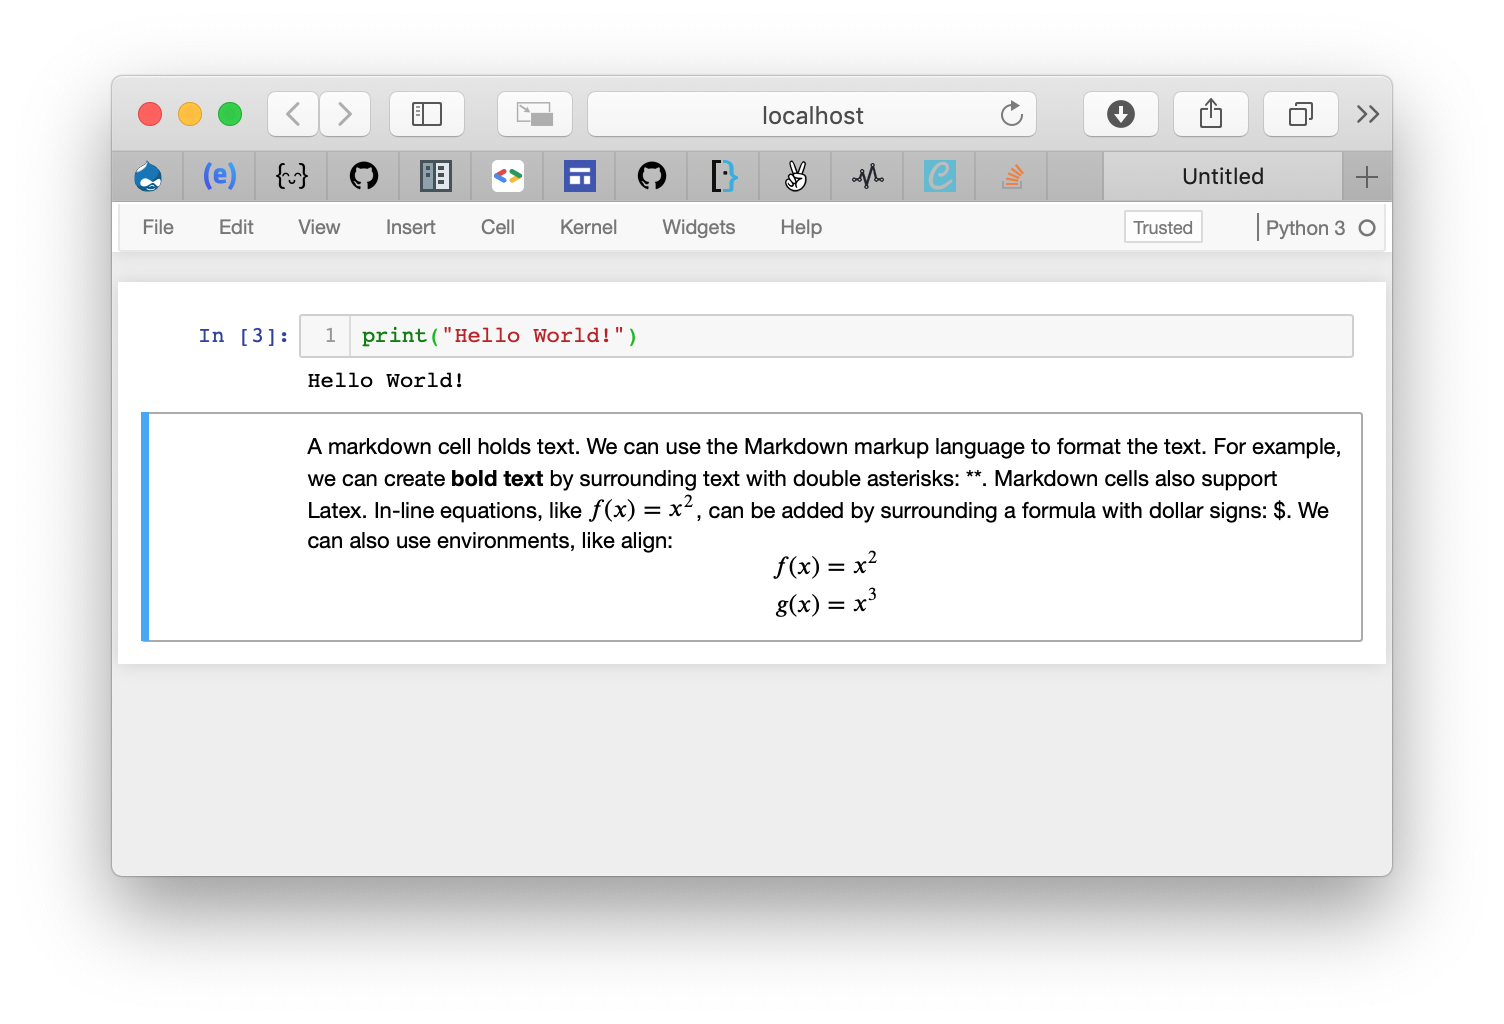
\includegraphics[width=.9\linewidth]{/Users/guilhermesalome/Teaching/Duke/Econ890 Python - 2019/supporting/python_markdown_cell.png}
\caption{\label{fig:orgdf01b9d}
Rendered Markdown Cell.}
\end{figure}

Notice that after hitting \texttt{Control-Enter} you exit \texttt{Edit Mode} and go into \texttt{Command Mode}.
You can edit the markdown cell by hitting \texttt{Enter} (going into \texttt{Edit Mode} again).
You can also hit \texttt{Shift-Enter} to format the text and create a new cell below it.

In \texttt{Command Mode} you can move between cells using the arrow keys up and down, or with the letters \texttt{j} (move down) and \texttt{k} (move up)\footnote{Using the letters \texttt{k} and \texttt{j} as shortcuts to move up and down come from the shortcuts of the text editor \texttt{Vim}. In \texttt{Vim} you move around text using the letters \texttt{h} (left), \texttt{j} (down), \texttt{k} (up) and \texttt{l} (right). This is a more efficient method of moving around text instead of using the arrow keys.}.
While in \texttt{Command Mode}, you can change a cell into a code cell with \texttt{y}, and into a markdown cell with \texttt{m}.
You can create a new cell above the current one with \texttt{a}, below the current one with \texttt{b}.
You can delete a cell with \texttt{d d}.
You can cut a cell with \texttt{x}, and paste it with \texttt{v}.
When using \texttt{v} to paste, the cell will be pasted below the current cell, but you can use \texttt{Shift-v} to paste the cell above.
You can copy a cell with \texttt{c}.
We can copy (or cut) multiple cells by first selecting many cells while holding \texttt{Shift} (for example, press \texttt{Shift-k} a few times), and then pressing either \texttt{c} or \texttt{x}.

In \texttt{Command Mode} you can toggle the line numbers with \texttt{l}.
If a cell has an output (like in a code cell than you just executed), you can toggle the visibility of the output with \texttt{o}.
To save the notebook, go to \texttt{Command Mode} and use the shortcut \texttt{Command-S}, or the menu \texttt{File} and button \texttt{Save as...} or \texttt{Save and Checkpoint}.

In \texttt{Edit Mode} on a code cell, you can create new lines by hitting \texttt{Enter} or \texttt{Control-o}.
You can move to the end of a line with \texttt{Control-e}, and to the beginning of a line with \texttt{Control-a}.
Notice that \texttt{Control-o} will create a new line below the current line if your cursor is at the end of the line.
Also, \texttt{Control-o} will create a new line above the current line if your cursor is at the beginning of the line.
Lastly, \texttt{Control-o} will split the line if your cursor is in the middle of the text in a line.

In \texttt{Edit Mode}, you can move around text using the arrow keys.
Alternatively, you can use \texttt{Control-f} to move forward one letter on a line, \texttt{Control-b} to move backwards one letter on a line, \texttt{Control-n} to jump to the next line, and \texttt{Control-p} to jump to the previous line\footnote{Using the shortcuts \texttt{Control-b}, \texttt{Control-f}, \texttt{Control-n} and \texttt{Control-p} to move the cursor around text comes from the shortcuts used on the text editor Emacs. This is a more efficient method of moving around text instead of using the arrow keys. In Emacs, this is also more natural since almost all commands rely on the \texttt{Control} key.}.
To delete a single letter after the cursor use \texttt{Control-d}.
You can use \texttt{Control-k} to delete text from the cursor to the end of the line.
To undo edits use \texttt{Command-Z}, and to redo edits use \texttt{Command-Shift-Z}.

In \texttt{Edit Mode}, you can indent the code with \texttt{TAB}. Alternatively, you can use \texttt{Command-]} to indent the code, and \texttt{Command-[} to dedent.
You can add a comment line with \texttt{Command-/}.

A helpful suggestion is to change the function of the \texttt{CAPS LOCK} key on your keyboard.
To make commands more natural, change the \texttt{CAPS LOCK} to \texttt{Control}.
This will allow you to quickly maneuver in \texttt{Edit Mode} using the keyboard shortcuts (and you will be one step closer to learning how to navigate on Emacs).

If you are on an Windows, the shortcuts might be slightly different due to the lack of a \texttt{Command} key.
You can always check the shortcuts for your system by going on the menu \texttt{Help} and clicking on the button \texttt{Keyboard Shortcuts}.

Now you know the basics of how to operate a jupyter notebook.
These shortcuts will only get natural if you use them.
It is natural to be slow at the beginning, but you should get quicker as you practice more and more.
Jupyter notebook is used in the industry and in research labs to share code and results among peers.
\section*{Summary}
\label{sec:orgc9d7dd5}
By the end of this lecture notes you should know:
\begin{itemize}
\item How to install Python with the installer
\item What are the main IDEs available for Python
\item How programs are found by the terminal and what the \texttt{PATH} variable represents
\item What is the idea behind a virtual environment
\item How to create a virtual environment with \texttt{virtualenv}
\item How to activate and deactivate the virtual environment
\item How to install packages with \texttt{pip}
\item How to launch Jupyter notebook
\item How to create code cells, markdown cells and many shortcuts for the Command Mode and Edit Mode
\end{itemize}
If you find any typos or issues with these notes, please send me an \href{mailto:guilhermesalome@gmail.com?subject=Feedback: Python: Topic: Setting Up}{email} with your feedback.
\section*{References}
\label{sec:orgaa60b58}
\begin{itemize}
\item \href{https://www.guilhermesalome.com/teaching/2018-empirical-methods-in-financial-econometrics/posts/lecture-14-installing-python.pdf}{Installing Python}
\item \href{https://www.guilhermesalome.com/teaching/2018-empirical-methods-in-financial-econometrics/posts/lecture-14-managing-versions.pdf}{Managing Python Versions}
\item \href{https://www.guilhermesalome.com/teaching/2018-empirical-methods-in-financial-econometrics/posts/lecture-15-jupyter-notebook.html}{Jupyter Notebook for Python}
\item \href{https://virtualenv.pypa.io/en/latest/}{Virtualenv}
\item \href{https://jupyter.org/install}{Jupyter Notebook}
\item \href{https://code.tutsplus.com/tutorials/understanding-virtual-environments-in-python--cms-28272}{Tracking Packages}
\end{itemize}
\end{document}